\label{chapter:ch2}
W poniższym rozdziale zawarty został krótki opis oka, analiza teoretyczna dziedziny okulografii, jak również zaprezentowano typy algorytmów wykrywania fiksacji wykorzystanych do przeprowadzenia badań. Na końcu tego rozdziału przedstawiono metody wyświetlania danych. Ten rozdział oparto głównie o prace \cite{Main}, \cite{EvaluationMethodology}, \cite{MachineLearning}.
\section{Opis ludzkiej gałki ocznej}
Zadaniem poniższej sekcji jest zaprezentowanie podstawowych terminów związanych z działaniem ludzkiego oka oraz jego budową. Krótka analiza oka została przygotowana zgodnie z pracą numer \cite{EvaluationMethodology}.\par
Jednym z najważniejszych organów w ludzkim ciele jest oko. Służy ono do dostarczania większości informacji dotyczących otoczenia w jakim się znajdujemy, oraz poszerzania wiedzy o świecie. Około 10\% komórek mózgowych jest zaangażowanych przy interpretacji oraz analizie sygnałów dostarczanych z tego narządu.\par
Prosty schemat oka został zaprezentowany na rysunku \ref{fig:budowaoka}.\par
Działanie oka polega na projekcji światła wpadającego do rogówki, najbardziej zewnętrznej część oka, poprzez źrenicę, która może być regulowana tęczówką w zależności od ilości promieni świetlnych. Następnie światło przechodzi przez soczewkę, która załamuje promienie świetlne, ciało szkliste, kończąc na wewnętrznej warstwie oka, nazywanej siatkówką. Składa się ona z dwóch typów fotoreceptorów:
    \begin{itemize}
        \item 6 milionów czopków
        \item 100 milionów pręcików
    \end{itemize} 
Czopki odpowiadają za widzenie fotopowe, pręciki za widzenie skotopowe. Widzenie fotopowe pozwala na rozpoznawanie kolorów (czerwony, zielony, niebieski) przy dobrym oświetleniu, które nie może być zbyt intensywne, ponieważ czopki mogą ulec przesyceniu. Widzenie skotopowe to możliwość obserwacji czarno-białego obrazu przy słabszym oświetleniu, jednak obraz nie jest tak dokładny jak przy widzeniu fotopowym. Przykład zakresu absorbcji fal świetlnych można zaobserwować na rysunku \ref{fig:czopki}.
\begin{figure}[H]
    \centering
    \captionsetup{justification=centering,margin=2cm}
    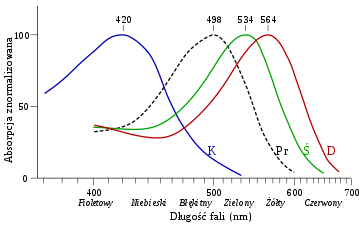
\includegraphics[width=0.9\linewidth]{resources/czopki.png}
    \caption[Względna absorbcja światła przez czopki oraz pręciki.]{Względna absorbcja światła przez czopki (K, Ś, D) oraz pręciki (Pr).\\\hspace{\textwidth}
    \small(źródło: \url{https://bit.ly/2WmM9qn} [dostęp 26.10.2019])}
    \label{fig:czopki}
\end{figure}
Na siatkówce pozyskany obraz jest obrócony względem rzeczywistego. Nerw wzrokowy transmituje dalej ten obraz jako sygnał nerwowy do ośrodków wzrokowych kory mózgowej. Ważnymi elementami przy poprawnie funkcjonującym oku są również ciało rzęskowe, posiadające promieniście ułożone fałdy, wydzielające wodnistą ciecz, odpowiadającą za sztywność gałki ocznej, jak również mięsień rzęskowy, który zmienia krzywiznę soczewki, co powoduje modyfikację jej ogniskowej, przez co występuje zjawisko akomodacji oka.
\begin{figure}[H]
    \centering
    \captionsetup{justification=centering,margin=2cm}
    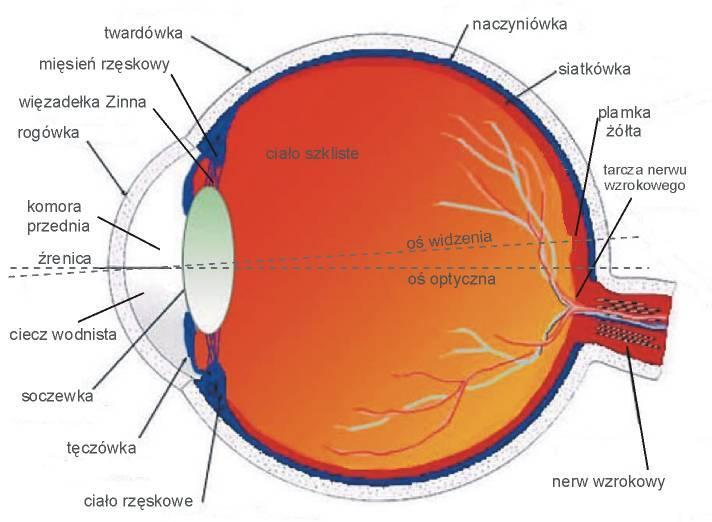
\includegraphics[width=0.8\linewidth]{resources/oko_galka.jpg}
    \caption[Przekrój oka.]{Uproszczony schemat gałki ocznej.\\\hspace{\textwidth} 
    \small(źródło: \url{https://eszkola.pl/fizyka/schemat-budowy-oka-i-wady-wzroku-4225.html} [dostęp 01.10.2019])}
    \label{fig:budowaoka}
\end{figure}
Akomodacja oka to zjawisko pozwalające oku na dostosowanie się do oglądania przedmiotów znajdujących się na różnych odległościach. Jak wspomniano wcześniej, fotoreceptory znajdujące się w oku pozwalają nam rozpoznać obraz ze światła wpadającego do oka.\par
Najważniejszym dla nas elementem siatkówki jest plamka żółta, posiadająca największą rozdzielczość otrzymywanego obrazu, ze względu na najwyższe stężenie czopków w ludzkim oku. Umożliwia ona ludziom np. czytanie tekstu. Im dalej od plamki żółtej, tym zwiększa się ilość pręcików, a przez to zmniejsza się dokładność obrazu.
\section{Metody wykrywania ruchu gałek ocznych}
\label{sec:movement}
Celem poniższej sekcji jest zademonstrowanie metod wykrywania ruchu gałek ocznych. Jednym z głównych kryteriów dla tych mechanizmów jest ich inwazyjność. Może ona powodować dyskomfort u badanego podmiotu, co w rezultacie może dać przekłamane wyniki, przez to, że użytkownik może zachowywać się mniej naturalnie. Wiele badań również wykazuje to, iż preferowane jest, żeby badano jak największą liczbę osób z małą znajomością tematyki śledzenia ruchu oka. Jest to spowodowane tym, iż badany może wykonywać inne ruchy niż te które wykonuje naturalnie. Ta sekcja bazuje na danych znalezionych w pracy \cite{metodyeyetrack}. Poniżej przedstawiono trzy główne metody mierzenia ruchu oka.\par
\subsection{Metody bazujące na soczewkach kontaktowych}
\label{ssec:lenses}
Ta kategoria sposobów mierzenia ruchu oka wymaga od badanego założenia na gałki oczne soczewek kontaktowych, posiadających lustra, bądź cewki z kablem, które okrążają soczewkę kontaktową. Te cewki są połączone do zewnętrznego systemu cewek magnetycznych. Pomiar odbywa się za pomocą wykrywania zmian sił pola magnetycznego. Pomimo większego rozwoju technologicznego, ze względu na inwazyjność całego rozwiązania, jak również konieczność unieruchomienia głowy w trakcie przeprowadzenia pomiarów, zaniechano korzystania z tego typu rozwiązań. Przykład takich metod pokazano na rysunku \ref{fig:soczewki}.
\begin{figure}[H]
    \centering
    \captionsetup{justification=centering,margin=2cm}
    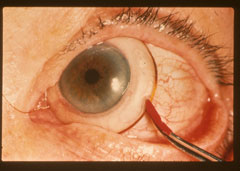
\includegraphics[width=0.9\linewidth]{resources/soczewki.png}
    \caption{Przykład rozwiązań bazujących na soczewkach kontaktowych.}
    \label{fig:soczewki}
\end{figure}
\subsection{Elektrookulografia}
\label{ssec:eog}
Elektrookulografia jest typem rozwiązań bazującym na różnicy potencjałów pomiędzy elektrodami przymocowanymi blisko oczu. Ze względu na dużą ilość połączeń nerwowych w gałce ocznej, można wykryć zmianę napięcia w samej gałce, gdzie wynosi ona około 1mV, jak również zauważalna jest zmiana pól elektrycznych podczas wykonywania ruchu. Amplituda tych zmian zależy od pozycji oka. Podobnie do rozwiązania prezentowanego w sekcji \ref{ssec:lenses}, to rozwiązanie straciło popularność na rzecz wideookulografii.
\subsection{Kamery}
\label{ssec:cameras}
Ostatnia, trzecia metoda pomiarów wykorzystuje kamery do rejestracji kolejnych pozycji ruchu. Ten sposób pozyskiwania danych wykorzystuje dwa typy obrazów: obraz z naturalnego światła oraz z podczerwieni. Obraz z naturalnego światła jest nazywany \emph{podejściem pasywnym}, które pobiera dane z odbitego światła z oka, wynikiem tego obrazu jest zarys ruchu soczewki. Te rozwiązania zaprezentowano poglądowo na rysunkach \ref{fig:camerassub1} i \ref{fig:camerassub2}. Jak można zaobserwować z rysunków, te metody nie wymagaja specjalnego montażu na użytkowniku. Z tego względu one znalazły najszersze zastosowanie w dziedzinie pomiaru ruchu gałek ocznych. Wadą tego rozwiązania jest zależność od źródła światła, gdyż pomiary przeprowadzane w złym świetle mogą powodować przekłamania, a w skrajnych przypadkach brak możliwości odczytu danych. Wykorzystanie odczytu światła podczerwieni eliminuje ten problem. Kolejną zaletą użycia podczerwieni jest zmiana wyniku, z zarysu ruchu soczewki na zarys ruchu źrenicy, poprzez wykorzystanie zjawiska odbicia światła z ekranu. W wypadku spojrzenia na element, odbicie jest rejestrowane jako biały punkt, w przeciwnym wypadku jako czarny punkt.
\begin{figure}[H]
    \centering
    \begin{subfigure}{.5\textwidth}
      \centering
      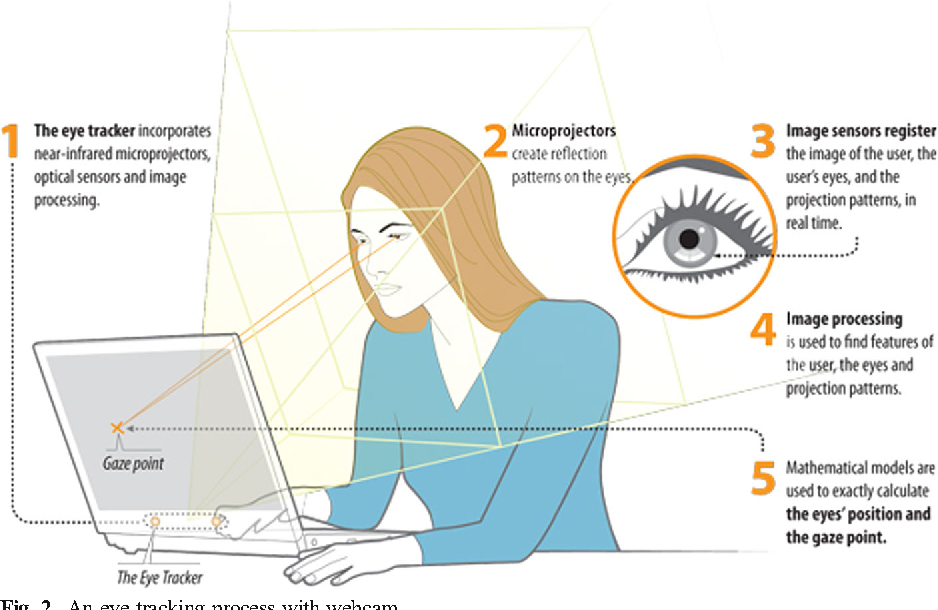
\includegraphics[width=\linewidth]{resources/camera.png}
      \caption{Stanowisko z kamerą}
      \label{fig:camerassub1}
    \end{subfigure}%
    \begin{subfigure}{.5\textwidth}
      \centering
      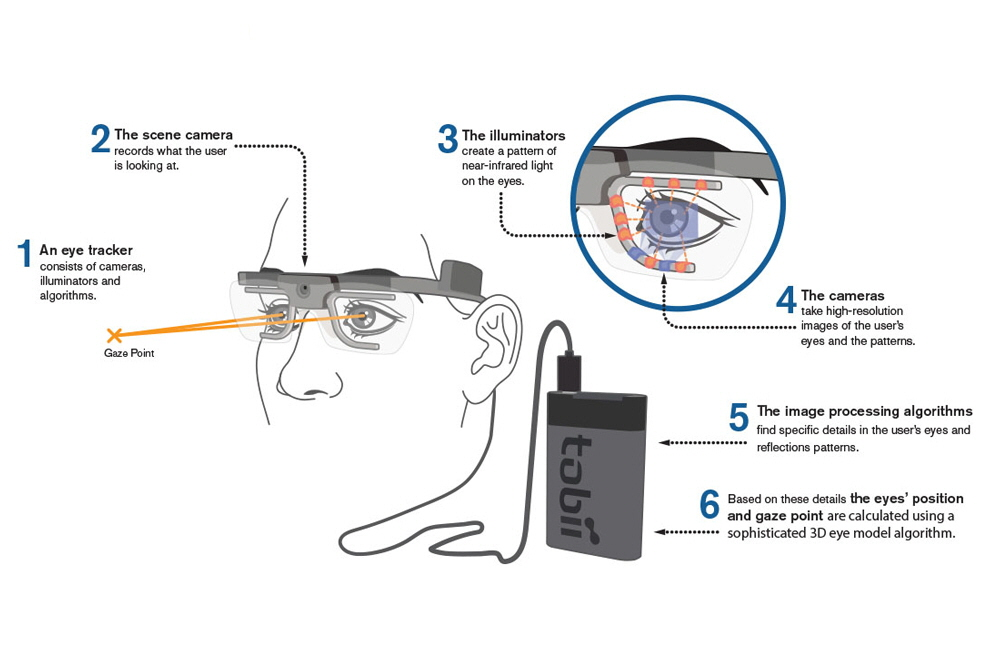
\includegraphics[width=\linewidth]{resources/glasses.jpg}
      \caption{Kamera w okularach}
      \label{fig:camerassub2}
    \end{subfigure}
    \caption[Przykłady zastosowania kamer]{Przykłady zastosowania kamer\\
    \small(źródło: \url{https://bit.ly/2NiZiwp} [dostęp 01.10.2019])}
    \label{fig:cameras}
\end{figure}
\section{Eye-tracking}
\label{sec:eyetracking}
W tej sekcji przybliżono technologię okulografii, oraz jej zastosowania.\par
Jak wspomniano we wstępie do pracy, rozwój omawianej dziedziny w przeciągu ostatnich kilkudziesięciu lat pozwala nam przeanalizować sposób w jakim operują ludzkie procesy obserwacji oraz sposobu rozpoznawania obrazu. Analiza tych procesów umożliwia badającym na wykorzystywanie wyników badań w zastosowaniach komercyjnych, np. badanie sposobu patrzenia na jezdnię, oraz deskę rozdzielczą w trakcie poruszania się pojazdem samochodowym \cite{CarSteering}, analiza psychologiczna \cite{GazeEyeTrackingSolutions} czy też w przygotowaniach do tworzenia reklam \cite{Advertising}.\par
W celu przetworzenia danych z urządzenia pomiarowego, których przykłady zaprezentowano w podrozdziale \ref{sec:movement}, do dalszej analizy stosuje się typowo dwie wartości: fiksacje, czyli miejsca, na których badana osoba się skupiła, oraz sakady, szybkie ruchy pomiędzy fiksacjami. Podział ten został odkryty w XIX wieku we Francji za pomocą obserwacji fizycznych, ponieważ zauważono, że ludzkie oko podczas czytania nie porusza się płynnie, a wykonuje "skoki" pomiędzy obszarami tekstu. Przykład takiego ruchu oraz punktów skupienia można zaobserwować na rysunku \ref{fig:fiksacje}.
\begin{figure}[H]
    \centering
    \captionsetup{justification=centering,margin=2cm}
    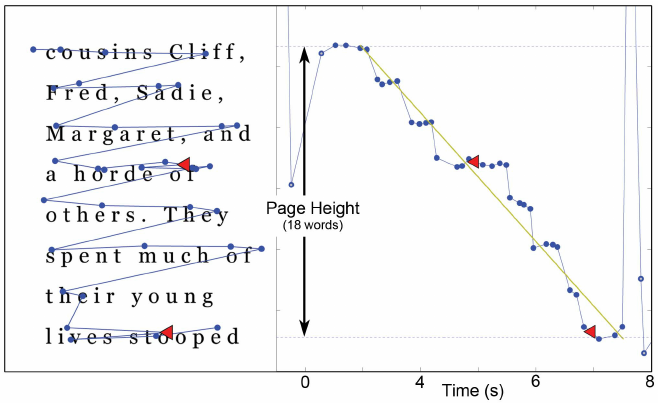
\includegraphics[width=0.8\linewidth]{resources/fixation_example.jpg}
    \caption[Przykład fiskacji i sakad na tle czytanego tekstu.]{Przykład fiskacji i sakad na tle czytanego tekstu.\\\hspace{\textwidth}
    \small(źródło: \url{https://upload.wikimedia.org/wikipedia/commons/e/ef/Reading_Fixations_Saccades.jpg} [dostęp 10.09.2019])}
    \label{fig:fiksacje}
\end{figure}
Analiza danych odbywa się między innymi poprzez translacje danych ruchu oka z urządzenia wejściowego na fiksacje, zezwalając na wykonanie podziału danych. Daje to możliwość pozbycia się mniej interesujących danych z próbki, takich jak sakad, pomniejszych ruchów oka, które mogły nastąpić przy niedokładnym pomiarze, czy przy mikroskopijnym ruchu oka. Cytując \cite{Main} \emph{"w większości badań naukowych, dane z sakad nie stanowią aż takiej przydatności"}. Zezwala to nam na zmniejszenie rozmiaru danych, poprzez zbijanie rzeczywistych fiksacji do jednego, większego punktu danych. Najczęściej otrzymane wartości są wykorzystywane do metryk pomiaru typu czas fiksacji, prędkości i amplitudy sakad, jak również miary pomiędzy fiksacjami a sakadami.\par
Wyniki algorytmów wykrywania fiksacji są wynikami typowo statystycznymi, tzn. możemy określić ile wystąpiło fiksacji, a przez to ile elementów jest sakadami, ale dalsza analiza danych należy do badającego. Stwarza to problem interpretacji danych, zgodnie z \cite{Main} \emph{"jednym ze sposobów walidacji tych algorytmów jest porównanie wynikowych fiksacji z wrażeniami wizualnymi obserwującego"}.
\section{Algorytmy wykrywania fiksacji}
\label{sec:fixations}
Wyróżniamy trzy typy algorytmów wykrywania fiksacji ze względu na badany obszar:
\begin{itemize}
    \item prędkościowe
    \item dyspersyjne
    \item powierzchniowe
\end{itemize} 
Algorytmem prędkościowym możemy nazwać algorytm, który analizuje punkty pod kątem różnicy prędkości pomiędzy nimi, biorąc pod uwagę, iż fiksacje posiadają niską prędkość pomiędzy swoimi punktami, a sakady wysoką. Algorytmy dyspersyjne bazują na odległościach pomiędzy punktami, zakładając, iż fiksacje posiadają małe odległości międzypunktowe. Algorytmy powierzchniowe to algorytmy, których zadaniem jest identyfikacja punktów w wybranych powierzchniach zainteresowania (AOI)\footnote{ang. area of interest}. Algorytmy tego rodzaju posiadają, w przeciwieństwie do innych algorytmów, możliwość identyfikacji zarówno nisko- jak i wysoko-poziomowej, przez to, iż parametrem algorytmów AOI może być fiksacja. Identyfikacja niskopoziomowa polega na pomiarze powierzchni wewnątrz jednej fiksacji, celem dokładniejszego podziału na fiksację i sakady.\\ 
Można także podzielić algorytmy ze względu na ich charakterystykę czasową, wyróżniamy dwa główne rodzaje:
\begin{itemize}
    \item czułe na czas trwania
    \item adaptujące się lokalnie
\end{itemize}
Ten podział został stworzony dlatego, iż fiksacje bardzo rzadko trwają mniej niż 100 ms, a regularny czas ich trwania potrafi wynosić od 200 ms do 400 ms. Implementacja adaptacji lokalnych umożliwia na dokładniejszy pomiar fiksacji, co znalazło zastosowanie w bardziej skomplikowanych algorytmach bazujących na międzypunktowych prędkościach ruchu oka i wyznaczonych obszarach zainteresowań
\subsection{Wybrane algorytmy}
\label{ssec:algorithms}
Celem poniższego podrozdziału jest opis teoretyczny algorytmów wykrywania fiksacji zastosowanych w pracy. Opis teoretyczny wybranych algorytmów bazuje na pracy \cite{Main} oraz \cite{EvaluationMethodology}.
\subsubsection{Algorytm I-VT}
\label{ssec:ivt}
Algorytm I-VT\footnote{z ang. Identification-Velocity Threshold} jest przykładem algorytmu z grupy prędkościowych. Jak wspomniano w podrozdziale \ref{sec:fixations} te algorytmy bazują na różnicach prędkości międzypunktowych. Przykładem tych różnic mogą być wartości mniej niż 150 stopni/sekundę dla fiksacji, a więcej niż 300-400 stopni/sekundę dla sakad. Ze względu na proste wymagania algorytmu, nie jest on skomplikowany w implementacji. Pseudokod algorytmu I-VT zaprezentowano w kodzie \ref{lst:ivtpseudocode}.
\begin{lstlisting}[language=Python, caption=Pseudokod algorytmu I-VT, label={lst:ivtpseudocode}]
    def ivt:
        Oblicz prędkości pomiędzy punktami dla wszystkich punktów w protokole
        Określ punkty poniżej progu jako fiksacje, a powyżej jako sakady
        Połącz wszystkie punkty fiksacji w grupy fiksacji, usuń wszystkie sakady
        Zmapuj każdą grupę fiksacji do punktu znajdującego się w środku każdej grupy
        return zmapowane punkty
\end{lstlisting}
Pierwszym krokiem algorytmu I-VT jest obliczenie prędkości między każdym punktem w badanym obszarze. Prędkość ta jest mierzona jako odległość między obecnym punktem a następnym (lub poprzednim) punktem. Następnie każdy punkt jest klasyfikowany jako fiksacja lub sakada w zależności od spełnienia warunku progu, którym w tym wypadku jest prędkość. Zgodnie z zasadami tego typu algorytmów, wszystkie elementy ponad granicą zaliczamy jako sakady, a resztę jako fiksacje. Kolejnym krokiem jest pozbycie się danych niepotrzebnych - sakad, i połączenie pozostawionych danych w grupy fiksacji. Ostatnim krokiem algorytmu jest wyznaczenie środka masy każdej grupy fiksacji, co pozwala nam zdefiniować fiksację jako punkt.\par
Według specyfikacji, ten algorytm posiada jeden parametr wewnętrzny, próg prędkości.
\subsubsection{Algorytm I-DT}
\label{ssec:idt}
\begin{lstlisting}[language=Python, caption=Pseudokod algorytmu I-DT, label={lst:idtpseudocode}]
    def idt:
        while istnieją punkty do zbadania:
            Zainicjalizuj okno na pierwszych punktach, celem pokrycia progu czasowego.
            if dyspersja punktów w oknie >= próg:
                Dodaj dodatkowe punkty do okna aż dyspersja > próg
                Zanotuj fiksacje jako centroid punktów w oknie
                Usuń punkty w oknie z listy punktów
            else:
                Usuń pierwszy punkt z listy punktów
        
        return fiksacje
\end{lstlisting}
Następnym badanym algorytmem jest algorytm uwzględniający rozproszenie punktów pomiaru ruchu okularach I-DT\footnote{z ang. Identification Dispersion-Threshold}. W przeciwieństwie do wcześniej omówionego algorytmu I-VT, algorytmu I-DT wykorzystuje fakt, iż fiksacje ze względu na swoją małą prędkość mają tendencje do grupowania się. Algorytm I-DT identyfikuje te fiksacje za pomocą okien (grup punktów) o określonej dyspersji (\emph{maksymalna separacja}). Pseudokod algorytmu można znaleźć w kodzie \ref{lst:idtpseudocode}.\par
Algorytm I-DT wykorzystuje ruchome okno, do którego należą punkty będące potencjalnymi fiksacjami. Zgodnie z powyższym pseudokodem, inicjalizacja okna następuje na podanym przez użytkownika progu czasowym. Następnie sprawdzana jest dyspersja pomiędzy punktami, którą można obliczyć za pomocą wzoru: $D = [max(x) - min(x)] + [max(y) - min(y)]$. Jest to wzór dla płaszczyzny dwuwymiarowej, jednak można zastosować inne wzory w wypadku użycia innych płaszczyzn przy wykonywaniu pomiaru. W wypadku gdy obliczona dyspersja przekroczyła zadany próg, nie znaleziono fiksacji, okno zostaje przesunięte na kolejny punkt. W przeciwnym wypadku okno należy zanotować jako fiksację. W tym oknie należy dodawać elementy aż obliczona dyspersja przekroczy próg dyspersji. Algorytm się kończy w momencie gdy wszystkie punkty zostaną przeanalizowane.\par
Algorytm I-DT wymaga podania dwóch parametrów wejściowych: progu dyspersji oraz progu czasowego. Ponieważ fiksacje zazwyczaj trwają mniej niż 100 ms, można określić próg czasowy na poziomie 150-200 ms. W wypadku znajomości kąta pomiędzy okiem a ekranem, możemy określić próg dyspersji w granicy $0.5^o$ do $1^o$ do znanej wartości. W innym wypadku należy określić przybliżoną wartość na podstawie eksploracji danych pomiarowych.
\subsubsection{Uczenie maszynowe}
\label{ssec:machinelearning}
W przeciągu ostatniej dekady można zauważyć znaczący wzrost zainteresowania technologiami powiązanymi z zagadnieniem sztucznej inteligencji, czy też uczenia maszynowego. Dzięki temu, iż dane wydobyte przez urządzenie śledzące ruch oka można łatwo sparametryzować, czy to przez podanie prędkości międzypunktowych, czy przez obliczanie dyspersji pomiędzy każdą parą punktów, również w dziedzinie eye-trackingu można zaobserwować wzrost wykorzystania technologii ML\footnote{Machine Learning}. Dla okulografii głównym wykorzystaniem tego typu rozwiązań jest możliwość automatycznej analizy danych, bez konieczności podawania parametrów wejściowych, takich jak w tradycyjnych algorytmach zaprezentowanych we wcześniejszych akapitach. Możliwość analizy danych bez parametrów eliminuje błędy powiązane z ich niepoprawnymi wartościami. Użycie tego sposobu wymaga od użytkownika podania już scharakteryzowanych danych, w wypadku wykrywania fiksacji jest to informacja, czy dany punkt należy do fiksacji, czy jest sakadą.\par
Opis działania algorytmu, jak również sposób analizy danych został zaprezentowany w sekcji \ref{ssec:machinelearningalg}.
\section{Metody prezentacji danych}
\label{sec:othereyetracking}
W oparciu o obliczone fiksacje, istnieje wiele rodzajów wizualnej analizy danych pochodzących z urządzenia mierzącego, na podstawie pracy \cite[rozdział 2.2]{OtherEyetrack}, możemy wykonywać tą analizę poprzez mapy cieplne, których przykład pokazano na rysunku \ref{fig:heatmap}. Mapy cieplne to obszary reprezentujące zwiększoną aktywność oka w danym miejscu, czy też punkty skupienia. Podobną metodą analizy danych są ścieżki skanowania, których zadaniem jest pokazanie linii, w jakich przebiega obserwacja na obrazie. Rysunek \ref{fig:scanpaths} ukazuje przykład ścieżek skanowania wraz z numeracją, jak przebiegał ruch oka. Metody te posiadają jednak pewne wady, mapy cieplne ukazują nam tylko pewną reprezentacje skupienia obiektu, nie ukazując nam kolejności w jakiej obraz został przeglądany. Ścieżki skanowania, jak zaprezentowano na rysunku \ref{fig:scanpaths} pozwalają zaprezentować dokładny przebieg badanej próbki na rysunku, jednak w wypadku zbyt dużego nagromadzenia danych, taki rysunek może być nieczytelny.
\begin{figure}[H]
    \centering
    \captionsetup{justification=centering,margin=2cm}
    \begin{subfigure}{.5\textwidth}
      \centering
      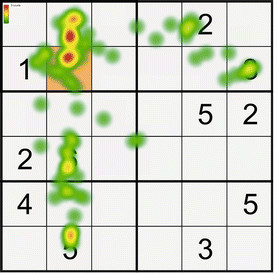
\includegraphics[width=\linewidth]{resources/heatmaps.png}
      \caption{Przykład mapy cieplnej}
      \label{fig:heatmap}
    \end{subfigure}%
    \begin{subfigure}{.5\textwidth}
      \centering
      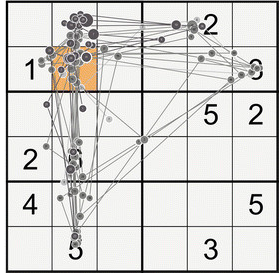
\includegraphics[width=\linewidth]{resources/scanpaths.png}
      \caption{Przykład ścieżki skanowania}
      \label{fig:scanpaths}
    \end{subfigure}
    \caption[Inne reprezentacje mierzonych punktów]{Inne reprezentacje mierzonych punktów.\\\hspace{\textwidth}
    \small(źródło: \url{https://bit.ly/2MZnIev}\footnote{ze względu na długi adres, należało skrócić link} [dostęp 10.09.2019])}
    \label{fig:otherfigures}
\end{figure}